

This section outlines our approach. The overall methodology is illustrated in figure

%Both static information and motion information, are correlated with the actions occurring in a video. For example, diving action
%is highly associated with swimming pools, and javelin throw is highly likely to happen in a scenario, where a sports field, a javelin and an athlete is
%present. Therefore, it is important to extract both static and motion information, in order to accurately predict and classify actions. In other words,
%individual objects, scene information, and actions and movements of actors and objects are extracted, in the process of prediction. 


%Also, a complex action may consist of smaller sub actions. For example, javelin throw action consists of sub events like getting ready,
%running, and throwing the javelin. Also, a specific order of sub events are associated with the complex action. 
%Therefore, it is important to investigate the evolution of sub activities with respect to time, in order to predict
%complex actions. We investigate this using following method. A video is segmented in to smaller segments, and features are engineered for each of these sub segments. A video can be then represented as a vector time series $C = [c_{t_0}, c_{t_1}, ...c_{t_{n-1}}]$.
%, where $n$ is the number of segments. Then, a recurrent neural net is applied on these features, to extract temporal dynamics.
\begin{figure*}
  \centering
  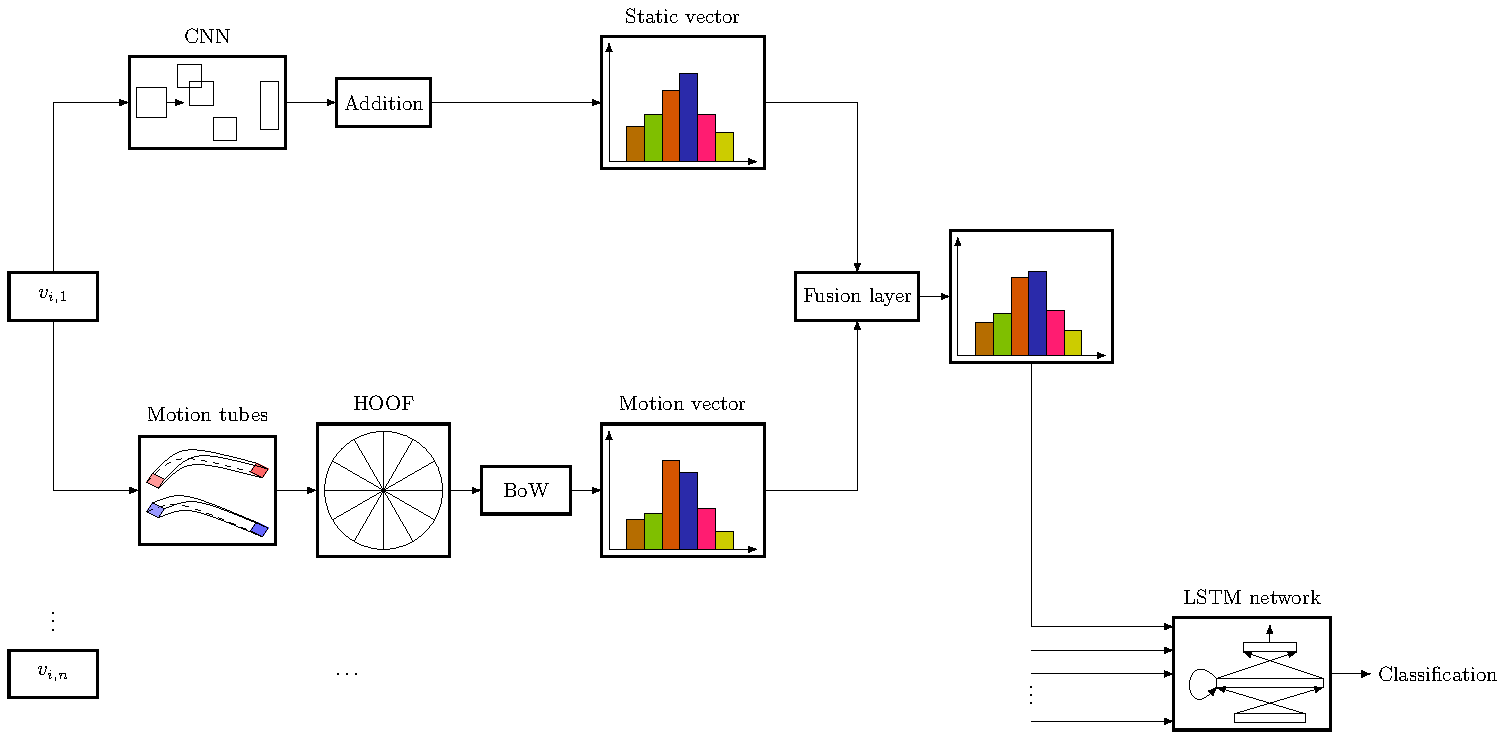
\includegraphics[scale=0.7]{overall.pdf} 
  \caption{Test Figure}\label{fi:test}
\end{figure*}


First, a video is segmented in to smaller segments, with a constant frame overlap, and features are engineered for each of these sub segments. 
We create features, for describing both motion and static domains.

For extracting motion features, we create \textit{motion tubes}, across frames, where we track each moving area along the frames, using action boxes.
Action boxes are square shaped regions, which contain significant motion, in each frame. These candidate areas are choosen by, first creating dense trajectories, for each frame,
and then clustering trajectory points, after a significant amount of pre processing. This process is explained in detail, in next section. 
These action boxes are linked across the frames to create motion tubes. Then, histogram oriented optic flows (HOOF) features are calculated within these motion tubes, and a 
\textit{bag of features}
method is applied on these features, to create a descriptor for each video segment. 

For extracting static features, we train a deep convolutional neural net, on the popular dataset Imagenet, and then apply this convolutional neural net,
on the frames of a video segment, to retrieve deep features from it. Then, these features are used
to create a static descriptor for the video segment.

Afterwards, we combine these features, using a mathematical model.

A video can then be represented as a vector time series $C = [c_{t_0}, c_{t_1}, ...c_{t_{n-1}}]$.
, where $n$ is the number of segments. Then, a recurrent neural net is applied on these features, and dynamics of time evolution of the combined vector are exploited,
by applying a recurrent neural net. Then, by classifying the dynamics of this time series, the actions are predicted.



